\setcounter{chapter}{1}
\chapter{          ÉTUDE PRÉLIMINAIRE}
\minitoc %insert la minitoc
\graphicspath{{Chapitre2/figures/}}

%\DoPToC

%==============================================================================
\pagestyle{fancy}
\fancyhf{}
\fancyhead[R]{\bfseries\rightmark}
\fancyfoot[R]{\thepage}
\renewcommand{\headrulewidth}{0.5pt}
\renewcommand{\footrulewidth}{0pt}
\renewcommand{\chaptermark}[1]{\markboth{\MakeUppercase{\chaptername~\thechapter. #1 }}{}}
\renewcommand{\sectionmark}[1]{\markright{\thechapter.\thesection~ #1}}

\begin{spacing}{1.5}

%==============================================================================
\section*{Introduction}
Après avoir présenté le cadre général de notre projet, nous entamons par le biais de ce chapitre une étude théorique, préface à sa réalisation. Nous commençerons par présenter les notions de base associées à la partie métier du projet. Nous enchaînerons avec l'étude de l'existant, qui sera l'opportunité de présenter plus en détail la problématique rencontrée en interne par l'entreprise. Enfin, une vue d'ensemble des solutions similaires présentes sur le marché permettra de se faire une idée globale sur les fonctionnalités à attendre du produit.\\
Cette étude, partie intégrale de l'élaboration de la vision initiale du produit, s'inscrit dans la phase d'inception de la méthodologie de travail adoptée.


%==============================================================================
\section{La Gestion de Projet}
Les entreprises se confrontent à de nombreux challenges au cours de leur évolution (adaptation à des contraintes externes, lancement de nouveaux services ou produits, intégration de nouveaux outils, mises à jour des processus, ...). Chaque défi est relevé sous forme de projet. Un projet est défini sous forme d'une suite d'actions délimitée dans le temps, en vue de produire un résultat spécifique, un produit, un service ou une nouvelle organisation.\\
La gestion de projet a pour vocation de relever ces défis en mettant en place une organisation et une planification de l’ensemble des activités visant à assurer l’atteinte des objectifs du projet (qualité, coûts, délais, ...), à effectuer leur suivi, anticiper les risques et les changements à mettre en œuvre  ainsi qu'à gérer la communication et la prise de décision.\\
\\
On peut regrouper les activités de gestion de projet en deux phases :
\begin{itemize}
%    \item \textbf{} :
    \item La phase d'organisation
    \item La phase de pilotage
\end{itemize}
\\
Ces activités sont précédées par une phase de collecte d'informations et d'étude de faisabilité. Cette phase d'avant projet permet de valider le projet et de décider des ressources à mobiliser pour sa mise en œuvre.
% REF: http://ressources.aunege.fr/nuxeo/site/esupversions/6b35be1e-5317-4cd6-8db2-05485615219d
% REF: http://www.gestiondeprojet.net
%-----------------------------------------------------------------------------------
\subsection{Phase d'organisation}
La phase d'organisation comprend le développement des concepts définis dans la phase d'avant projet et la définition du référentiel du projet, en fournissant suffisamment de détails pour pouvoir entamer la phase de réalisation. Les principaux éléments du référentiel d'un projet incluent :
\begin{itemize}
%    \item \textbf{} :
    \item \textbf{La charte du projet} : Elle est rédigée par le chef de projet dès son lancement. Elle est destinée à toutes les personnes appelées à travailler sur le projet, ainsi qu'aux tiers concernés (la hiérarchie, les chefs de service, ...). C'est un document de référence à usage strictement interne dont le but est de fournir les informations de base du projet : son objet, ses parties prenantes, ses enjeux, ses contraintes, etc.
    \item \textbf{La structuration du projet} : La structure de découpage du projet organise et définit la totalité du contenu d'un projet. La structuration du projet dépend de nombreux paramètres (la complexité, la structure de l'organisation, le type de gestion, ...) et a pour objectif de découper le projet en plus petits éléments, plus faciles à gérer, afin de pouvoir définir des coûts et des durées pour chaque élément, ainsi que des résultats tangibles et mesurables.
    \item \textbf{Le planning de référence} : La planification d'un projet est l’activité qui consiste à déterminer et à ordonnancer les tâches du projet, à estimer leurs charges et à déterminer les profils nécessaires à leur réalisation. Le planning résultant inclut la liste des tâches et leurs antériorités, la définition des lots de travaux ainsi que les ressources associées.
    \item \textbf{Le plan de communication} : C'est un document qui présente les méthodes et les modalités adoptées pour collecter, conserver et diffuser l'information, les destinataires de chaque type d'information (rapport, document technique, ...), ainsi que les responsabilités associées.
    \item \textbf{Le budget de référence} : Résultat de l'analyse des coûts rattachés au projet, il est établi à partir de la liste des activités, des ressources associées et du planning de référence.
    \item \textbf{L'analyse des risques} : Elle comporte un recensement des aléas majeurs associés au projet ainsi que les plans d'action et les mesures préventives à mettre en place.
\end{itemize}

%-----------------------------------------------------------------------------------
\subsection{Phase de pilotage}
Une fois budgétisé, organisé et planifié, le projet démarre. Le pilotage du projet permet de comparer le réalisé avec le prévisionnel, et de réviser éventuellement les plannings et les charges. Le chef de projet et son équipe s'efforcent de respecter le référentiel de gestion du projet, tout en mesurant les écarts constatés. Cela inclut la maîtrise des aspects suivants :
\begin{itemize}
%    \item \textbf{}} :
    \item \textbf{Les délais} : Le chef de projet recueille l'information sur l'avancement réel du projet à partir de l'avancement de chaque tâche, et identifie les retards actuels et potentiels. Dès lors, des actions correctives peuvent être mises en place afin de corriger les écarts (modification du planning, réallocation de ressources, ...).
    \item \textbf{Les coûts} : Une évaluation de la consommation budget est fréquemment entreprise, suivie d'une réestimation du budget qui reste à consommer. Le coût total prévu comparé au budget de référence permet d'analyser et d'anticiper des écarts ainsi que d'identifier les causes de dépassement.
    \item \textbf{Les modifications} : Elles sont le résultat d'événements extérieurs (changement de réglementation, changement demandé par le client, erreurs ou oublis dans la définition initiale, ...). Les demandes de changements peuvent apparaître sous plusieurs formes et conduire à un élargissement ou à une limitation du contenu et doivent être traitées grâce un ensemble de procédures formelles.
    \item \textbf{Les risques} : La maîtrise des risques permet d'identifier, de quantifier, de réduire ainsi que de suivre les risques encourus tout au long de la vie du projet.
\end{itemize}
Le chef de projet se focalise essentiellement sur la maîtrise des coûts et des délais.\\

L'usage d’indicateurs de pilotage est crucial pour le pilotage efficace d'un projet. Ces outils d'assistance à la décision permettent de mesurer de manière pratique une situation ou un risque, d'alerter ou au contraire de signifier l'avancement correct d'un projet.


%==============================================================================
\section{Étude de l'existant}
L'étude de l'existant permet d'identifier les points forts ainsi que les points faibles de la solution existante. Cette étude permettra de bien cibler les besoins de l'entreprise, en vue d'en tenir compte lors de la conception et du développement de la solution.
%-----------------------------------------------------------------------------------
\subsection{Description de l'existant}
La solution de gestion de projet actuelle se base sur l'utilisation du logiciel Excel pour générer des documents associés aux différentes activités d'un projet. En effet, le chef de projet répertorie chaque catégorie d'artéfact associée à la gestion d'un projet sous forme de tableur Excel. Il procède ainsi à l'ajout et l'édition d'entrées pour chaque catégorie d'artéfact et y indique l'ensemble des informations requises. Cette procédure est facilitée par la duplication de fiches Excel de base, vierges, préparées à l'avance pour chaque catégorie. Ainsi, pour chaque catégorie d'artéfact, l'ensemble des entêtes et des valeurs prédéfinies pour chaque champs y est déja déclaré. La table d'entrées d'une fiche est souvent accompagnée d'un ensemble d'indicateurs, statiques et dynamiques, pertinents à la catégorie en question. Des exemples de ces fiches sont exposés aux figures \ref{fig:risqueFiche} et \ref{fig:actionFiche}, traitant respectivement des artéfacts actions et risques pour un projet.

\begin{figure}[H]
\centering
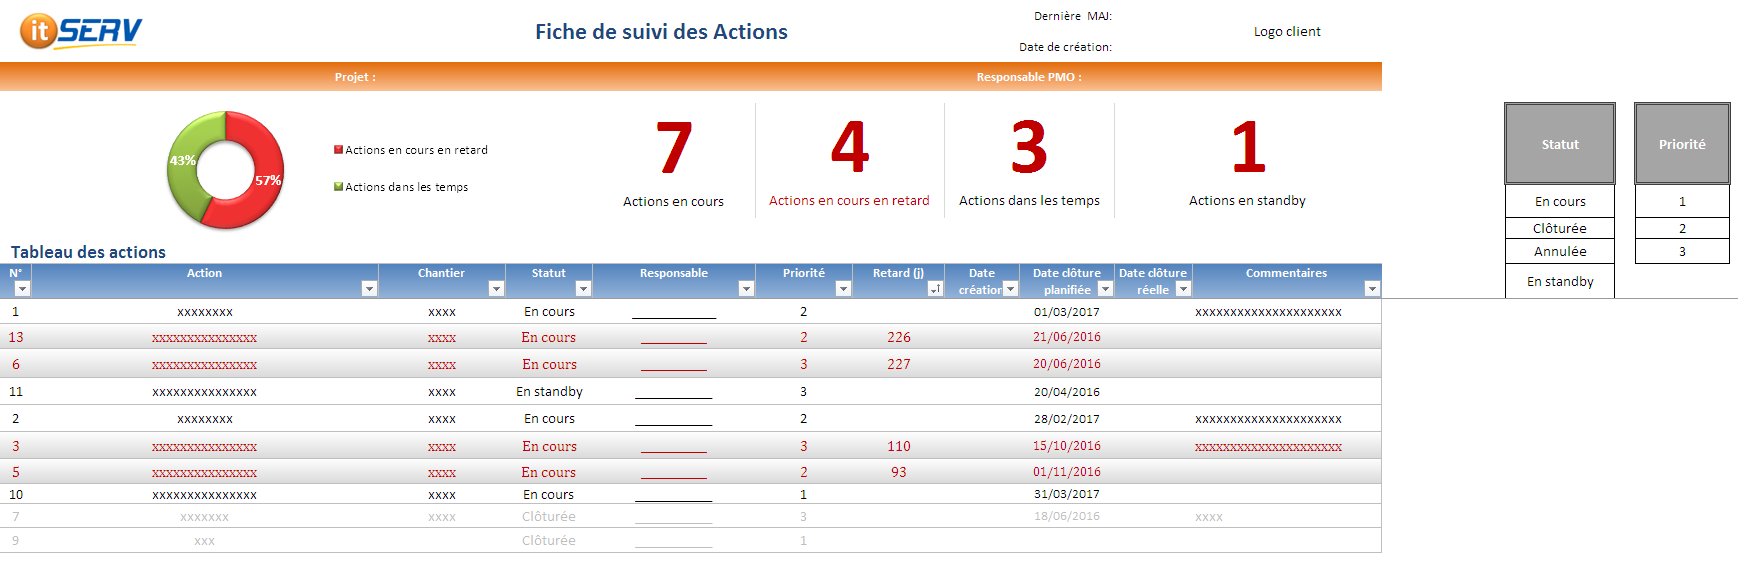
\includegraphics[width=\linewidth]{ficheActions.png}
\caption{Exemple d'une fiche de suivi des actions}
\label{fig:actionFiche}
\end{figure}

\begin{figure}[H]
\centering
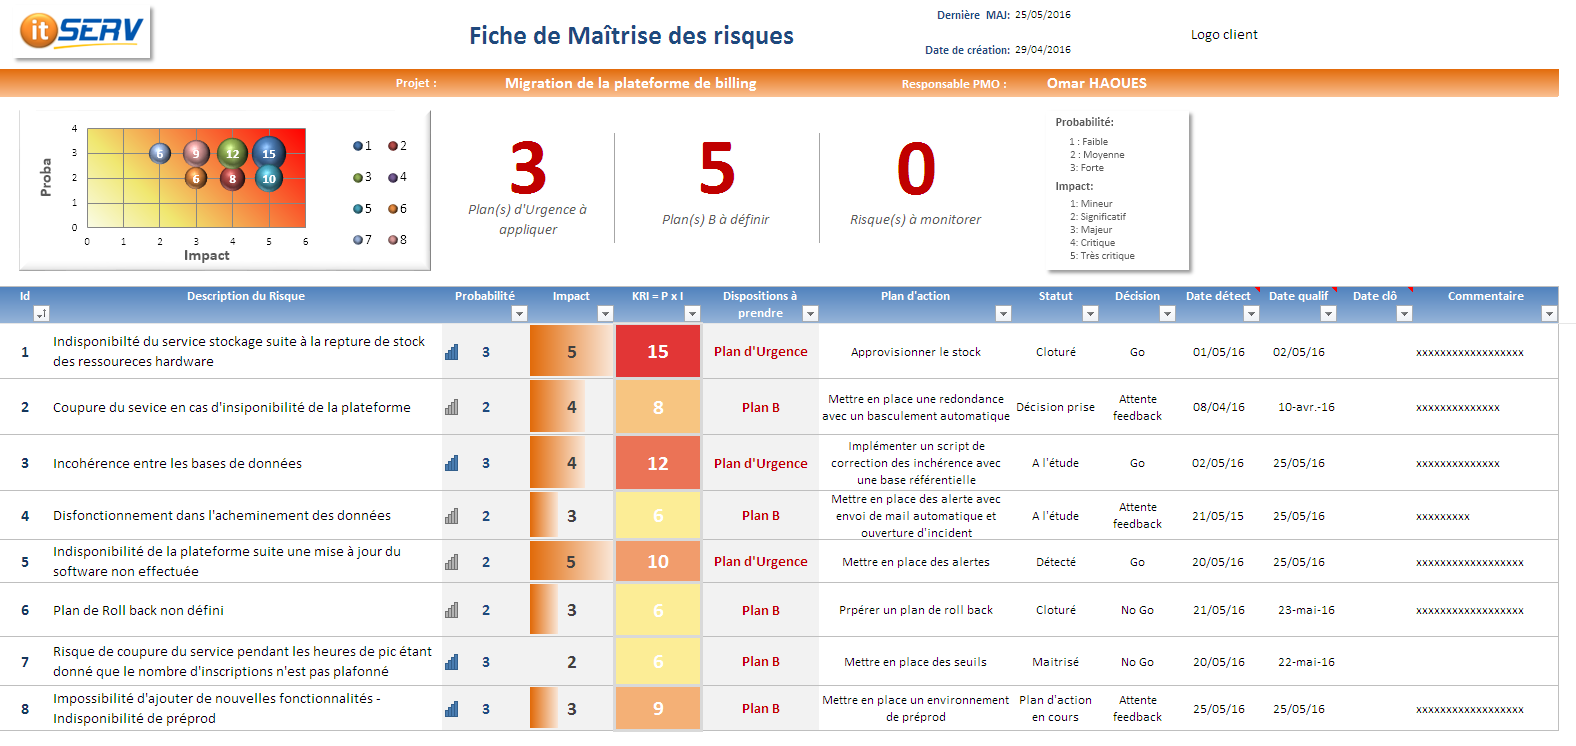
\includegraphics[width=\linewidth]{ficheRisques.png}
\caption{Exemple d'une fiche de maîtrise des risques}
\label{fig:risqueFiche}
\end{figure}
\

Le chef de projet est régulièrement chargé de diffuser les mises à jour relatives à un projet, périodiquement ou à la demande, au travers de l'envoi de messages électroniques directement aux parties concernées.\\

Cette méthode de travail possède certains atouts, mais dissimule dans l'ensemble plusieurs inconvenances qui nuisent à son niveau d'efficacité et à la performance de la gestion de projets par l'entreprise. Ces points sont exposés dans la section suivante.

%-----------------------------------------------------------------------------------
\subsection{Critique de l'existant}
La présentation de la méthode de gestion actuelle nous permet de déceler des limitations importantes, inhérentes à la démarche générale.\\
\\
Reconnaissons tout d'abord les mérites non négilgeables de celle-ci, à savoir :
\begin{itemize}
    \item Disponibilité de fiches de base, contraignant les champs à choix restraints aux options prédéfinies et assistant à leur remplissage
    \item Présence de champs autocalculés ainsi que de supports visuels utiles pour la compréhension de certains champs, dont la signification peut s'avérer obscure
    \item Génération automatique d'indicateurs riches (statistiques numériques, graphiques en camembert, ...)
\end{itemize}
\

Outre ces quelques bénéfices, cette méthode de gestion présente les nombreuses limitations suivantes :
\begin{itemize}
    \item \textbf{Perte en productivité} : induite d'un déficit d'automatisation de la démarche de gestion des fichiers
    \item \textbf{Fragmentation des données} : les données relatives à chaque projet sont réparties, sous forme d'une multitude de documents, souvent désorganisés
    \item \textbf{Journalisation non fiable des mises à jour} : la journalisation des mises à jours relève entièrement de l'organisation choisie par le chef de projet, et requiert un effort manuel, exclusivement dédié à la tâche
    \item \textbf{Traçabilité impossible} : l'origine des modifications des fichiers n'est pas connue
    \item \textbf{Stockage inneficace} : problème de centralisation pour l'ensemble des données des projets menés par l'entreprise, redondance de données, oraganisation manuelle, etc
    \item \textbf{Sécurité non garantie} : la sécurisation des données (documents) est entièrement à la charge des parties prenantes y ayant accès
    \item \textbf{Condifentailité difficile à assurer} : elle implique en pratique l'édition soigneuse, au cas par cas, des fichiers partagés
    \item \textbf{Synthèse des données impossible} : impossible de se reposer fiablement sur les données des fichiers pour les besoins d'aide à la décision de l'entreprise (à cause des points susmentionnés)
    \item \textbf{Collaboration fastidieuse} : contribution d'intervenants non gérée par la solution actuelle. Le chef de projet transforme individuellement tous les flux d'information en données, avant de les indiquer dans le fichier approprié
\end{itemize}
\

Toutes les limitaions susmentionnées imposent pour l'entreprise une révolution dans sa méthode actuelle de gestion de projets. Dans le cadre de notre projet de fin d'études, la solution à concevoir aspire ainsi à combiner les points forts de la démarche existante tout en apportant une solution efficace à ses problèmes inhérents.


%==============================================================================
\section{Étude des solutions existantes sur le marché}
Le problème de gestion de projet est aussi vieux que le concept de projet lui-même. En conséquence, un nombre important de solutions logicielles d'aide à la gestion de projet est disponible aujourd'hui sur le marché. Dans le but de produire une solution de qualité, une étude de l'existant s'impose afin de prendre en considération les points forts et les points faibles des solutions existantes. Celle-ci servira surtout à nous guider dans l'élaboration de la vision de notre produit.

%-----------------------------------------------------------------------------------
\subsection{Présentation des solutions existantes}
Les solutions présentes sur le marché se distinguent les unes des autres essentiellement par le niveau de fonctionnalités offert et le domaine d'application cible. En effet, des solutions populaires, telle que JIRA \ref{JIRA}, se limitent à un domaine très particulier, en l'occurence la gestion de projets agiles pour cette dernière. Les solutions étudiées aspirent à être le plus générique possible, capable d'être employées dans n'importe quel contexte de projet. L'échantillon exposé ci-dessous vise à présenter une vue d'ensemble des caractéristiques communes et distinctives des solutions les plus populaires sur le marché qui partagent cette vision.

\subsubsection*{MS Projects} %-------------------------------------------------------------------------
Microsoft Projects a su s'imposer pendant longtemps en tant que solution de facto pour les besoins de gestion de projet en entreprise. Faisant partie de la suite logicille de l'éditeur, MS Projects ne fait pas exception et s'intègre pleinement à sa plateforme collaborative \ref{Office 365}, ce qui représente un réel bénéfice pour les clients ayant déja opté pour l'intégration de leurs données sur cette dernière. Le logiciel continue d'introduire un nombre de fonctionnalités avancées avec ses mises à jour. Ceci le rend particulièrement adapté aux besoins poussés de gestion de projet. Les utilisateurs expérimentés y trouvent leur compte, cependant la courbe d'apprentisage est souvent pénible pour les novices et s'avère être trop complexe pour les usages se limitant en besoin à un nombre restreint de ses fonctionnalités.

\subsubsection*{ProjectManager.com} %------------------------------------------------------------------
ProjectManager.com couvre très bien les fonctionnalités de base de gestion de projet et, parmi toutes les solutions étudiées, s'apparente le plus à la vision initiale élaborée. Cette solution, disponible sous une offre SaaS \ref{SaaS}, s'adapte parfaitement aux besoins des petites et moyennes entreprises, qui retrouvent une simplicité d'usage associée à une couverture plus que décente des piliers de la gesion professionnelle de projet.

\subsubsection*{Zoho Projects} %-----------------------------------------------------------------------
Zoho propose une suite logicielle qui répond aux besoins des particuilers et des entreprises. Dans cette optique, sa solution de gestion de projet s'intègre parfaitement avec certains de ses autres produits, afin d'étendre ses fonctionnalités. La solution se veut simple, mais complète, en offrant un éventail éttoffé de fonctionnalités pour la gestion des divers facettes d'un projet. Elle se caractérise par une attention particuière apportée à l'ergonomie et au confort général d'utilisation.

\subsubsection*{EasyProject (EasyRedmine)} %-----------------------------------------------------------------------------
Redmine est la solution open source gratuite la plus complète disponible sur le marché. Cependant, son manque d'intuitivité et le faible niveau d'ergonomie offert, associés à son interface datée, nuisent à son potentiel et en font une solution peu courante d'usage dans la pratique. C'est tout d'abord dans le but d'accroître son utilisabilité, tout en prenant avantage de la base de fonctionnalités existante, que la solution EasyProject offre une version commerciale, basée sur cette solution. Depuis, l'application s'est vu évoluer vers l'une des solutions les plus abouties du marché, visant à s'aligner avec les standards de gestion de projets IPMA et PMI.

\subsubsection*{Clarizen} %-----------------------------------------------------------------------------
Due à l'amélioration continue de son produit et à la complétude de sa vision, l'entreprise Clarizen a vu son produit se hisser à la position de Leader dans dans les classements Gartner et Forrester de 2016 \ref{clarizen.com}, dans la catégorie des solutions SaaS de gestion de projets. De ce fait, ce produit a sans nul doute sa place dans notre étude et impose un bilan des traits caractéristiques qui lui valent son succès.
\\

Dans le but de présenter un échantillon pertinent, d'autres solutions ont été omises, notamment pour des raisons de redondance ou de pauvreté en termes de fonctionnalités. Nous poursuivons avec la mise en relief des points communs et distinctifs de chacune dans la partie qui suit.

%-----------------------------------------------------------------------------------
\subsection{Synthèse des solutions existantes}

Le tableau \ref{tab:} présente une comparaison haut niveau des solutions étudiées. On y observe que les solutions retenues partagent un tronc commun de fonctionnalités destiné à la gestion des aspects primordiaux d'un projet. Elles se différencient néanmoins sur d'autres points, tel que la nature de l'offre et le support de l'accès mobile.

\begin{table}[h]
\centering
\caption{Comparatif des solutions de gestion de projet présentées}
\label{comparatifSolutionsEtudiees}
\begin{tabularx}{1\textwidth}{|p{4cm}|1|1|1|1|1|}
\hline
        \textbf{Spécificités} & \textbf{MS Proj.} & \textbf{P.M .com} & \textbf{Zoho Proj.}&  \textbf{EasyProject} & \textbf{Clarizen}\\
\hline
        \textbf{Nature d'offre} & Bureau & SaaS & SaaS & SaaS \& Local & SaaS\\
\hline
		\textbf{Planification} & \cmark & \cmark & \cmark & \cmark & \cmark\\
\hline
		\textbf{Gestion Budget} & \cmark & \cmark & \cmark & \cmark & \cmark\\
\hline
		\textbf{Structuration} & \cmark & \cmark & \cmark & \cmark & \cmark\\
\hline
		\textbf{Gestion Ressources} & \cmark & \cmark & \cmark & \cmark & \cmark\\
\hline
		\textbf{Gestion Problèmes} & \cmark & \cmark & \cmark & \cmark & \cmark\\
\hline
        \textbf{Gestion} & \multirow{2}{*}{\xmark} & \multirow{2}{*}{\cmark} & \multirow{2}{*}{\cmark} & \multirow{2}{*}{\cmark} & \multirow{2}{*}{\cmark}\\
        \textbf{Modifications} &  &  &  &  & \\
\hline
		\textbf{Reporting} & \cmark & \cmark & \cmark & \cmark & \cmark\\
\hline
		\textbf{GED} & \cmark & \cmark & \cmark & \cmark & \cmark\\
\hline
		\textbf{Pilotage Risques} & \cmark & \cmark & \cmark & \cmark & \cmark\\
\hline
		\textbf{Support Mobile} & \xmark & Web & App & App & App\\
\hline
		\textbf{Collaboration} & \xmark & \cmark & \cmark & \cmark & \cmark\\
\hline
		\textbf{Open Source} & \xmark & \xmark & \xmark & \cmark & \xmark\\
\hline
\end{tabularx}
\end{table}
\

Vu son expertise en développement d'applications, IT SERV a choisi de démarrer le développement de sa propre solution d'aide à la gestion de projet. Dans le cadre de notre projet de fin d'études, nous visons à concevoir une solution s'inspirant d'une sélection des traits jugés primordiaux des solutions étudiées. Ceux-ci seront établis dans le chapitre \ref{chap: spécs}.

%==============================================================================
\section*{Conclusion}
Afin de mieux cerner la problématique et de proposer une solution de qualité, tenant compte des spécificités de notre projet, nous avons établi l'état des lieux de l'existant, que ce soient les méthodes de gestion courantes de l'entreprise, ou les solutions similaires disponibles sur le marché.\\
Avec ces informations en main, le chapitre suivant nous permettra de dégager précisément les exigences de notre produit.


%==============================================================================
\end{spacing}
